\section{Methods}
In this section we first describe the dataset used in our work in detail. We then describe the baseline model as well as models used in our experiments. We close with an overview of the data pre-processing needed to match the models’ architectures.

\subsection{Dataset}
\label{dataset}
We use the melanoma segmentation dataset as published in the 2018 Lesion Boundary Segmentation Challenge by the International Skin Imaging Collaboration (ISIC) \citep{isic-2018-segmentation}. The dataset comprises dermatoscopic images with their corresponding ground truth segmentation masks \citep{ensambles-2016-codella}.

\par
The \emph{lesion} images were acquired by different dermatoscope types from several institutions, taken from all anatomic sites and from a historical sample of patients presented for skin cancer screening. Every image contains exactly one primary lesion. The distribution of disease states represent a modified "real world" setting (over-representation of malignancies) containing more benign lesions than malignant \citep{isic-2018-segmentation}.

\par
The ground truth is represented by binary segmentation masks which indicate the location of the primary skin lesion within each input image. The masks are represented by a single-channel 8-bit continuous region, where each pixel is either 0 (background - area outside of the primary lesion) or 255 (foreground - area inside the primary lesion) and have the exact same dimensions as the lesion images. The ground truth images were obtained using several techniques (e.g. fully automated algorithm; manual polygon tracing by human expert annotators), but all data were reviewed by practicing dermatologists with expertise in dermoscopy \citep{isic-2018-segmentation,ensambles-2016-codella}.

\par
The dataset is divided into train, validation and test sets with 2’594, 100 and 1’000 images respectively. The train and validation datasets contain the exact same number of ground truth segmentation mask images whereas the test dataset does not. The test dataset is used for the final evaluation of the challenge submission and hence does not contain any segmentation masks. In order to compensate for the reduced dataset, we used extensive data augmentation techniques like vertical and horizontal flips, random rotation (0-40 degrees), translation, shearing, color jittering, adding noise (gaussian distribution) and adding artificial hairs to in order to make the models more robust against hair occlusion while preserving the same static dataset distributions. The final dataset comprises 2’700 train images, 300 validation images and 300 original test images. Figure \ref{data_augmentation} shows the result of various data pre-processing and augmentation techniques.

\begin{figure}[ht]
  \centering
  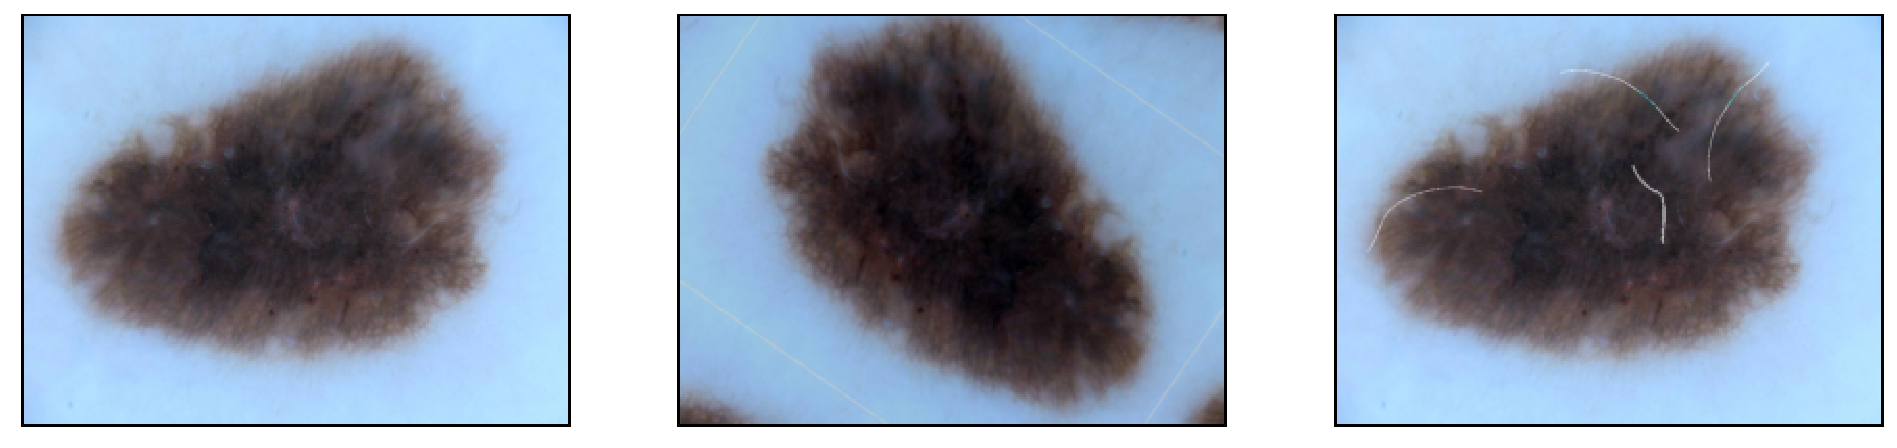
\includegraphics[width=\columnwidth]{assets/data_augmentation.pdf}
  \caption[Datasets]
  {Data augmentation: (left) original image, (middle) rotated image with additional augmentation like vertical flip, random scale, random brightness etc., (right) augmented image with artificial hair added.}
  \label{data_augmentation}
\end{figure}

The images in each dataset show a spectrum of variations in terms of quality (e.g. sharpness, lighting conditions, coloring etc.) and added noise (e.g. hair, rulers, bubbles etc.). Furthermore, the resolution of the images varies significantly. The \emph{train} dataset has 206 different dimensions, ranging from a resolution of 540 x 722 pixels to 4'499 x 6'748 pixels. The \emph{validation} dataset has 21 different resolutions, ranging from 480 x 640 pixels to 4'461 x 6'641 pixels. Lastly, the \emph{test} dataset has 114 different resolutions, ranging from 480 x 640 pixels to 4'519 x 6'808 pixels. Figure \ref{lesion_images} shows three examples of lesion images and their corresponding binary segmentation masks.

\begin{figure}[ht]
  \centering
  \includegraphics[width=\columnwidth]{assets/lesion_images.pdf}
  \caption[Lesion Images]
  {Three lesion images with different noise on the top with their corresponding binary masks at the bottom.}
  \label{lesion_images}
\end{figure}


\subsection{Models}
This section describes the baseline model and the model selections used in experiments in detail.

\subsubsection{Baseline}

We use U-Net \citep{unet-2015-ronneberger} with a VGG16 backbone (feature extractor) as our baseline model. The U-Net architecture was specifically designed for medical segmentation tasks and has been widely adopted as a baseline model in research.



\subsubsection{CNN \& Transformer based Models}

To address our hypothesis, we use different model architectures and model compositions from both CNN and Transformer deep neural network classes.

\par
We use five different flavours of the U-Net as CNN based models. The flavours differ mainly in the feature extractor used for the encoder part of the U-Net. Specifically, we use VGG16, Densenet121, EfficientNet0, Efficientnet4 and inceptionv3 as backbones. We also initialize the U-Net encoder with weights pre-trained on ImageNet which leads to an overall better performance. All model setups use the sigmoid activation function for the last layer with the number of segmentation classes set to 1  for binary image segmentation.

\par
For Transformer based models we used the Medical Transformer and TransUNet architecture. Medical Transformer is an encoder-decoder architecture which adds an additional control mechanism called Gated Axial-Attention in the self-attention module (encoder) as well as a Local-Global training strategy. This strategy helps the model to operate on the whole image resolution where it learns high-level features by modelling long-range dependencies (global), and on image patches which helps to focus on finer local features at the same time (local).

\par
TransUNet combines the merits from U-Net and Transformers to develop an architecture which gives local as well as global attention. It uses a CNN-Transformer Hybrid as an encoder along with skip-connections at different layers to leverage the localized attention from the CNN feature map in the decoding path.


\subsection{Data Pre-processing}
As discussed in section \ref{dataset} in detail the provided images show a variety of different resolutions, quality, general lighting condition and added noise like hair. In order to input the image to the models a pre-processing had to be done. Even though models like U-Net are image size agnostic meaning they can handle any resolution provided enough computational resources, we resize the input images to a fixed size appropriate to the selected model for training. To harmonize the image resolution, we use OpenCV’s resize method with INTER\_NEAREST interpolation. This allows for batching and hence faster training. Given the time and computational limits we perform an ablation study to determine the best image resolution for our experimental setup. Further, we normalize the input images to values between 0 and 1 (float64) to fit the models’ requirements. Image resizing and normalization are performed on the fly using our custom data loader implementation.


% \begin{itemize}
%   \item Define your task in a clear, concise manner
%   \item Formally describe each model under investigation. Include your baseline and experimental models at minimum.
%   \item For each model, describe its infrastructure and assumptions (if applicable).
% \end{itemize}
